\documentclass[acmtoms]{acmtrans2m}

\newtheorem{theorem}{Theorem}[section]
\newtheorem{conjecture}[theorem]{Conjecture}
\newtheorem{corollary}[theorem]{Corollary}
\newtheorem{proposition}[theorem]{Proposition}
\newtheorem{lemma}[theorem]{Lemma}
\newdef{definition}[theorem]{Definition}
\newdef{remark}[theorem]{Remark}

\usepackage{amsmath}
\usepackage{amsfonts}
\usepackage{float}
\usepackage{graphicx,wrapfig}
\usepackage{path}
\usepackage{moreverb}
\usepackage{color}

\newcounter{algorithm}
\renewcommand\thealgorithm{\thesection.\arabic{algorithm}}
\newenvironment{algorithm}[2]
{
  \begin{center}
    \noindent
    \framebox{\hbox{
        \begin{minipage}{5in} \refstepcounter{algorithm}
          \vspace{5pt}
          {{\sc Algorithm} \thealgorithm:
            \textsf{\bfseries{#1}} % \hfill \mbox{ ~ }
            } {
            \slshape #2 }
        \end{minipage}
        }}
  \end{center}
  }

%\newcommand{\aspace}[1]{Anasazi::#1}
\newcommand{\aspace}[1]{\texttt{#1}}

\newcommand{\cbcomm}[1]{\textcolor{blue}{\emph{#1}}}
\newcommand{\fin}[1]{\textcolor{red}{\emph{#1}}}

\markboth{C. G. Baker et al}{Anasazi software for the numerical
solution of large-scale eigenvalue problems}

\title{Anasazi software for the numerical solution of large-scale eigenvalue problems}

\author{C. G. Baker and
U. L. Hetmaniuk and R. B. Lehoucq and H. K. Thornquist\\ Sandia
National Laboratories}

\begin{abstract}
Anasazi is a package within the Trilinos software project that
provides a framework for the iterative, numerical solution of 
large-scale eigenvalue problems. Anasazi is written in ANSI C++ and
uses modern software paradigms to enable the research and development
of eigensolver algorithms. Furthermore, Anasazi provides implementations
for some of the most recent eigensolver methods.
The purpose of our paper is to describe the design and
development of the Anasazi framework. A performance comparison 
of Anasazi and the popular FORTRAN 77 code ARPACK are given. 
\end{abstract}

\category{G.1.3}{Numerical Analysis}{Numerical Linear Algebra}
\category{G.4}{Mathematical Software}{} \category{D.2.13}{Software
Engineering}{Reusable Software}

\terms{Algorithms, Design, Performance; Reliability, Theory}

\keywords{Eigenvalue problems, Numerical Algorithms, Generic
programming}

\begin{document}

\begin{bottomstuff}
Sandia is a multiprogram laboratory operated by Sandia Corporation,
a Lockheed Martin Company, for the United States Department of
Energy under contract DE-AC04-94AL85000. Authors' addresses: C. G.
Baker, U. L. Hetmaniuk, R. B. Lehoucq,
Sandia National Laboratories, Computational Mathematics \&
Algorithms, MS 1320, P.O.Box 5800, Albuquerque, NM 87185-1320; email
\{cgbaker,ulhetma,rblehou\}@sandia.gov. H. K. Thornquist, Sandia National
Laboratories, Electrical and Microsystem Modeling, MS 0316,
Albuquerque, NM 87185-0316; email hkthorn@sandia.gov.

\end{bottomstuff}

\maketitle

Anasazi is a package within the Trilinos
Project~\cite{Heroux:2005:OTP} that uses ANSI C++ and modern software
paradigms to implement algorithms for the numerical solution of
large-scale eigenvalue problems. We define a
large-scale eigenvalue problem to be one where a small number
(relative to the dimension of the problem) of eigenvalues and the
associated eigenspace are computed, and only knowledge of the
underlying matrix via application on a vector (or group of vectors)
is assumed.

An inspiration for Anasazi is the ARPACK~\cite{lesy:98} FORTRAN 77 software library.
ARPACK implements one algorithm, namely an implicitly restarted Arnoldi
method~\cite{sore:92}. In contrast, Anasazi provides a software framework, including the
necessary infrastructure, to implement a variety of algorithms. We justify our claims by
implementing block variants of three popular algorithms: a Davidson~\cite{morganscott:86} method,
a Krylov-Schur~\cite{stew:01} method, and an implementation of LOBPCG~\cite{knya:01}.

ARPACK has proven to be a popular and successful FORTRAN 77 library
for the numerical solution of large-scale eigenvalue problems. A
crucial reason for the popularity of ARPACK is the use of a reverse
communication~\cite[p.~3]{lesy:98} interface for applying the
necessary matrix-vector products. This allows ARPACK to provide a
callback for the needed matrix-vector products in a simple fashion
within FORTRAN 77. Unfortunately, the reverse communication
interface is cumbersome, challenging to maintain, and does not allow
data encapsulation. Moreover, because ARPACK uses a procedural
programming paradigm where the matrix-vector operations rely upon
the physical representation of the data manipulated, ARPACK is
susceptible to design changes. Hence, code reuse is limited and
software complexity and maintenance are more cumbersome.

The Anasazi framework employs more modern software development paradigms, both generic and
object-oriented programming, via static and dynamic polymorphism~\cite[Chapter 14]{VJ02}, respectively. 
Static polymorphism, via templating of the linear algebra objects, allows algorithms in Anasazi
to be written in a generic manner (i.e., independent of the data types). Dynamic
polymorphism, via virtual functions and inheritance, allows eigensolvers to be decoupled
from mechanisms such as orthogonalization and stopping conditions. Upshots of this
decoupling are the facilitation of code reuse, increased algorithmic flexibility, and the
ability to choose components at runtime.

We emphasize that our interest is not solely in modern software paradigms. Rather, our
paper demonstrates that a rich collection of block eigensolvers is easily implemented
using modern programming techniques. Our approach is algorithm-oriented \cite{muov:94}, in
that requirements for efficient implementations of the necessary algorithms is considered
first. This is then followed by a formulation of the software abstractions capable of
implementing these algorithms, and their constituent mechanisms, in sufficiently diverse
ways. The result is a collection of implementations that are efficient and flexible. We
believe that Anasazi is the natural successor to ARPACK, inheriting and extending the
quality practices employed by ARPACK.

There are related software efforts that implement several algorithms for solving
large-scale eigenvalue problems (the reader is referred to~\cite{slepc:05}
for a software survey).  The two most advanced, comparable software efforts are PRIMME and
SLEPc:
\begin{itemize}
\item
The Preconditioned Iterative Multi-Method Eigensolver (PRIMME)~\cite{primme:06} is a C
library for computing a number of eigenvalues and their corresponding eigenvectors of a real
symmetric or complex Hermitian matrix. PRIMME provides a highly parametrized
Jacobi-Davidson~\cite{slvo:96} iteration, allowing the behavior of multiple eigensolvers
to be obtained via the appropriate selection of parameters;
\item
The Scalable Library for Eigenvalue Problem Computations (SLEPc)~\cite{slepc:06} library
is another C library for the solution of large scale sparse eigenvalue problems on parallel
computers. SLEPc is an extension of the popular PETSc~\cite{petsc-web-page} and can be
used for either Hermitian or non-Hermitian, standard or generalized, eigenproblems.
\end{itemize}

PRIMME provides a flexible metasolver capable of implementing a variety of
Hermitian eigensolvers. Predefined parameters are provided to emulate a large number of powerful 
and popular eigensolvers, allowing easy use of the software by novice users. Expert users may
manually specify the parameters in order to access the full flexibility available in the
solver's behavior. Therefore, PRIMME is valuable both as a convenient eigensolver for
practitioners and a platform for experimentation by eigensolver researchers. However,
while parameters are provided to control mechanisms such as, e.g., stopping conditions and
orthogonalization, the user is limited to the implementations provided by the developers of
PRIMME.  Furthermore, PRIMME provides implementations only over double precision real and complex
fields.  Support for \texttt{float} or extended precision scalar fields would require separate
implementations due to the lack of generic programming ability in the C programming
language.

SLEPc extends the PETSc toolkit to provide a library of solvers for standard or
generalized, Hermitian or non-Hermitian eigenproblems.
SLEPc provides wrappers for several eigensolver packages, most notably ARPACK and PRIMME,
as well as native implementations of eigensolvers like Krylov-Schur, Arnoldi, and Lanczos.
The use of PETSc also gives SLEPc users access to a large library of linear and nonlinear 
solvers, preconditioners and matrix formats. PETSc uses C language features such as 
\texttt{typedef}s and function pointers to support some generic programming and object-oriented 
paradigms. However, SLEPc's reliance on PETSc requires that the user employ PETSc for vectors 
and matrices. Similar to PRIMME, SLEPc can be compiled with support for double precision
real or complex arithmetic, however only one version of the library can be used at a time.
Furthermore, mechanisms such as orthogonalization are hard-coded allowing only parametrized 
control over their behavior. 

The Anasazi framework was designed to include features from other eigensolver packages
that are conducive to algorithm development, while avoiding some of the drawbacks
mentioned above.  The most important features that have been incorporated into its design
are extensibility and interoperability.  The extensibility of the Anasazi framework is
demonstrated through the infrastructure's support for a significant class of large-scale
eigenvalue algorithms.  Extensions can be made through the addition of, or modification
to, existing algorithms and auxiliary functionality such as orthogonalization, desired
eigenvalue selection, and stopping conditions.  This is encouraged by promoting code
modularization and multiple levels of access to solvers and their data. 

Interoperability in the Anasazi framework is enabled via the treatment of both matrices and 
vectors as opaque objects---only knowledge of the matrix and vectors via elementary operations 
is necessary. This permits algorithms to be implemented in a generic manner, requiring no
knowledge of the underlying linear algebra types or their specific implementations.
Furthermore, the Anasazi framework was designed to admit operation with any user choice
of scalar field, vector and operator. This is accomplished using the template mechanism in
the C++ programming language, an option not available to SLEPc or PRIMME. As a result, an
Anasazi eigensolver using single-precision complex arithmetic can be used alongside
another Anasazi eigensolver using an extended precision scalar type. 

As a result of these design features, the Anasazi eigensolver framework is significantly
more flexible than previous efforts, allowing its inclusion in diverse application
environments in addition to providing an arena for research into eigensolvers and their
constituent mechanisms.  The rest of this paper is organized as follows.
Section~\ref{sec:algorithm-overview} briefly discusses one class of algorithms that can be
implemented using Anasazi in order to explore the types of operations necessary for an
eigensolver framework.  Section~\ref{sec:framework} reviews the Anasazi framework,
discusses some of the design decisions, and illustrates the benefits of these decisions.
Lastly, Section~\ref{sec:benchmarking} provides some timings comparing ARPACK and Anasazi
to demonstrate that object-oriented overhead has no impact on the performance of this
modern software framework.


\section{Algorithmic Inspiration}
%%%%%%%%%%%%%%%%%%%%%%%%%%%%%%%%%%%%%%%%%%%%%%%%%%%%%%
\label{sec:algorithm-overview}

The Anasazi software framework provides tools that are useful for solving a wide variety
of eigenvalue problems. While development of the package continues to expand its scope to
other important eigenvalue problems (e.g., nonlinear eigenproblems, constrained
eigenproblems), the solvers currently released with the package are aimed at computing a
partial eigen-decomposition for the generalized eigenvalue problem
\begin{equation}  \label{eq:intro.1}
  \mathbf{A} \mathbf{x} = \mathbf{B} \mathbf{x} \lambda , \qquad
  \mathbf{A}, \mathbf{B} \in \mathbb{C}^{n\times n}\ .
\end{equation}
In this paper, the matrices $\mathbf{A}$ and $\mathbf{B}$ are large, possibly sparse, and
we assume that only their application to a block of vectors is required. The reader is
referred to~\cite{saad:92,sore:02,stew:01book,vors:02} for background information and
references on the large-scale eigenvalue problem.

\begin{figure}[htb]
\begin{algorithm}{Rayleigh-Ritz Algorithm\label{algo:obliqueRR}}
{\smallskip
\begin{tabbing}
(nr)ss\=ijkl\=bbb\=ccc\=ddd\= \kill {\rm (1)} \>\> Let the matrix
$\mathbf{M}$ and bases $\mathbf{U}$, $\mathbf{V}$ be given
\\
{\rm (2)} \>\> Form the Rayleigh quotients $ \mathbf{V}^H
\mathbf{M}\Phi(\mathbf{A}) \mathbf{U}$ and $ \mathbf{V}^H \mathbf{M}
\Psi(\mathbf{B}) \mathbf{U}$\\
\>\> where $\Phi(\cdot)$ and $\Psi(\cdot)$ are matrix functions
\\
{\rm (3)} \>\> Compute an eigen-decomposition $(\mathbf{L},\mathbf{W})$ for the Rayleigh
quotients\\
\>\>\>\>$ \left(\mathbf{V}^H \mathbf{M}\Phi(\mathbf{A}) \mathbf{U}\right) \mathbf{W} = 
\left(\mathbf{V}^H \mathbf{M}\Psi(\mathbf{B}) \mathbf{U}\right) \mathbf{W} \mathbf{L}$
\\
{\rm (4)} \>\> Use the approximation $(\mathbf{L},\mathbf{W})$ and the basis $\mathbf{U}$
to construct \\
\>\>an approximation for the pencil $(\mathbf{A}, \mathbf{B})$
\\
\end{tabbing}
}
\end{algorithm}
\end{figure}

Algorithm~\ref{algo:obliqueRR} is a simple extension of the Rayleigh-Ritz procedure given
in~\cite[p.284]{stew:01book}. This algorithm lists the salient steps found in the majority
of large-scale eigensolvers, namely subspace projection methods.  The matrices $\mathbf{U}$ and
$\mathbf{V}$ are bases for the trial and test subspaces $\mathcal{U}$ and $\mathcal{V}$, 
respectively.  When these two subspaces are distinct, then the Rayleigh-Ritz method is called
oblique.  Otherwise, when $\mathcal{V}=\mathcal{U}$ the orthogonal Rayleigh-Ritz method results.
The functions $\Phi(\cdot)$ and $\Psi(\cdot)$ are often used to improve convergence to the 
eigenvalues and eigenspace of interest.  The matrix $\mathbf{M}$ is often used to denote an 
inner product; for instance $\mathbf{M}$ can be set equal to $\mathbf{A}$ or $\mathbf{B}$ when
either matrix is Hermitian positive semi-definite.

The Rayleigh-Ritz procedure is useful for
examining some of the functionality that should be provided by a general eigensolver
framework.  However, first we should observe some general structure of the participants in
this algorithm.  The bases $\mathbf{U}$ and $\mathbf{V}$ are dense matrices that are stored
as a collection of vectors, which we call a \emph{multivector}.  Interaction with 
$\mathbf{A}$, $\mathbf{B}$, and $\mathbf{M}$ requires only knowledge of the underlying matrix
via application on a vector or multivector, thus we regard these matrices as \emph{operators}.
The functions $\Phi(\cdot)$ and $\Psi(\cdot)$ should also be considered operators and, while the
choice of functions is outside the scope of this
paper, the use of these types of operators should not be hindered.  

Given these observations,
the functionality that is important to an eigensolver includes:
\begin{itemize}
  \item multivector creation: create $\mathbf{U}$, $\mathbf{V}$
  \item operator-multivector applications: $\Phi(A)U$, $\Psi(B)U$;
  \item multivector arithmetic: $\mathbf{V}^H\mathbf{U}$;
  \item solution of typically much smaller eigenproblems (step~3).
\end{itemize}
A full list of our primitives for operators and multivectors will be presented in Section \ref{sec:framework}. 
It is worthy to note at this point that the Anasazi framework was designed to support block methods,
defined as those that apply $\mathbf{A}$ or $\mathbf{B}$ to a collection of vectors, or multivector.
One advantage of using a multivector data structure is that it can improve the ratio of 
floating-point
operations to memory references and so better exploit a memory hierarchy.

\begin{figure}[htb]
\begin{algorithm}{Eigen-iteration\label{algo:eigen-iter}}
{\smallskip
\begin{tabbing}
(nr)ss\=ijkl\=bbb\=ccc\=ddd\= \kill {\rm (1)} \>\> Update the
bases $\mathbf{U}$ and $\mathbf{V}$\\
{\rm (2)} \>\> Determine whether any portion of the
eigen-decomposition\\
\>\> is of acceptable accuracy
\\
{\rm (3)} \>\> Deflate the accurate portions of the
eigen-decomposition
\\
{\rm (4)} \>\> Terminate the eigen-iteration or return to step (1).
\\
\end{tabbing} }
\end{algorithm}
\end{figure}

Algorithm~\ref{algo:obliqueRR} needs to be augmented with several steps in order
to result in an \emph{eigen-iteration}. Algorithm \ref{algo:eigen-iter} lists these
additional steps and allow us to further analyze the
components that make up an eigen-iteration.  
The decisions involved in Steps~2 and 4 require the determination of the interesting portion of the
eigen-decomposition and a definition of accuracy or algorithmic breakdown, thus they are 
likely candidates for decoupling from the
implementation of a particular eigen-iteration. For a particular eigen-iteration,
deflation (Step~3) also may be conducted in a manner of ways. Steps~1 and 3, whatever their
implementation, typically require orthogonalization methods, which are an active area of research.
These methods provide another opportunity for decoupling functionality that need not be
implemented in a specific manner.



% The matrices $\mathbf{U}$ and $\mathbf{V}$ are bases for the trial
% and test subspaces $\mathcal{U}$ and $\mathcal{V}$, respectively.
% When these two subspaces are distinct, then the Rayleigh-Ritz method is
% called oblique. Otherwise, when $\mathcal{V} = \mathcal{U}$ the
% orthogonal Rayleigh-Ritz method results. The functions $\Phi(\cdot)$
% and $\Psi(\cdot)$ are often used to improve convergence to the
% eigenvalues and eigenspace of interest. For example, a standard
% approach is to reformulate equation (\ref{eq:intro.1}) as
% $$
% %\begin{equation}  \label{eq:si}
%   \Phi(\mathbf{A}) \mathbf{x} \equiv
%   (\mathbf{A}- \mathbf{B}\sigma)^{-1}\mathbf{B}\mathbf{x} =  \mathbf{x}
%   (\lambda-\sigma)^{-1} \equiv \Psi(\mathbf{B})\mathbf{x} \nu ,
% %\end{equation}
% $$
% where $\nu=1/(\lambda-\sigma)$ is the eigenvalue of the reformulated
% system and $\sigma \in \mathbb{C}$ is near the 
% eigenvalues of interest.
% This is an example of the shift-invert spectral transformation. The
% matrix $\mathbf{M}$ is often used to denote an inner product; for
% instance $\mathbf{M}$ can be set equal to $\mathbf{A}$ or
% $\mathbf{B}$ when either matrix is Hermitian positive semi-definite.
% A second example is to apply an equivalence transformation to
% (\ref{eq:intro.1}) resulting in
% $$
%    \Phi(\mathbf{A}) \mathbf{x} \equiv
%    \mathbf{N}^{-1}\mathbf{A} \mathbf{x} = \mathbf{N}^{-1}\mathbf{B} \mathbf{x} \lambda
%    \equiv \Phi(\mathbf{B})\mathbf{x}\lambda
% $$
% where $\Psi = \Phi$ and set $\mathbf{M}=\mathbf{N}$.

% Of
% course, the assumption is made that linear systems with $\mathbf{A}-
% \mathbf{B}\sigma$ can be solved, either with a sparse direct method
% or a preconditioned iterative method.
% We define the \emph{eigenproblem} as (\ref{eq:intro.1}) and the
% \emph{eigen-operator}, or simply operator, as $OP$. Examples of the
% latter are $OP = \mathbf{A}$ or $OP = (\mathbf{A}-
% \mathbf{B}\sigma)^{-1}\mathbf{B}$. $OP$ will often utilize a
% preconditioned iterative method\footnote{We refer the reader
% to~\cite{Arbenz:2005:ACE} for an involved discussion of several
% approaches to solving the symmetric positive semi-definite
% (\ref{eq:intro.1}).}.


% A distinguishing characteristic of the Rayleigh-Ritz algorithm is
% the number of columns $m$ of $\mathbf{U}$ and $\mathbf{V}$. The size of the
% bases $\mathbf{U}$ and $\mathbf{V}$ is either constant or
% increasing. An example of the former is the gradient-based method
% LOBPCG~\cite{knya:01}. Examples of the latter are the Davidson
% algorithm~\cite{davi:75} and Krylov-based methods such as the
% Arnoldi~\cite{arno:51} and Lanczos~\cite{lanc:50} methods.
% Ultimately, the success of an algorithm depends crucially upon these
% subspaces and the choice of bases representation, an issue that is
% beyond the scope of this paper.

%The algorithms that are currently available in Anasazi are:
%\begin{enumerate}
%  \item a block extension of a Krylov-Schur method~\cite{stew:01},
%  \item a block Davidson method as described in~\cite{Arbenz:2005:ACE},
%  \item an implementation of LOBPCG as described in~\cite{Hetmaniuk:2006:BSL}.
%\end{enumerate}

% removed the first two of these remarks; they do not add
% anything to the paper and may distract the reader. re-emphasize that
% this section was simply an exploration of one type of eigensolver
% strategy, intended to demonstrate some of the primitive operations
% which should be provided by an eigensolver framework (this should be
% said at the beginning as well). keep the third point but expand: block
% eigensolvers provide numerous benefits.

% Three remarks are in order. First, all three algorithms are
% instances of the orthogonal Rayleigh-Ritz method. Therefore the
% eigen-decomposition computed in step $(3)$ of
% Algorithm~\ref{algo:obliqueRR} is equivalent to a Schur form when
% (\ref{eq:intro.1}) is a regular pencil.
% 
% Our second remark is that only the Krylov-Schur method can be used
% for non-Hermitian generalized eigenvalue problems. In contrast, all
% three algorithms can be used for symmetric positive semi-definite
% generalized eigenvalue problems.

This discussion illustrates that many distinct parts make up a
large-scale eigensolver code: orthogonalization, sorting tools, dense
linear algebra, convergence testing, multivector arithmetic, etc.
Anasazi presents a framework of algorithmic components, decoupling
operations where possible in order to simplify component verification,
encourage code reuse, and maximize flexibility in implementation.

%Our
%resulting implementations are therefore backward stable. Such a
%reliance allows us to conclude that we have computed a nearby
%partial Schur decomposition. The distance to the problem of interest
%is then bounded by the size of residual associated with the computed
%Schur decomposition.
%\begin{table}[htb]
%\caption{Necessary steps when implementing Algorithm
%\ref{algo:obliqueRR}} \label{table:additional-steps}
%\begin{center}
%\begin{tabular}{|ll|}\hline
%(1)& maintaining a basis $\mathbf{U}$ that is orthonormal to working
%precision\\
%(2) & restarting the iteration (need to define) when the number of
%basis vectors in $\mathbf{U}$ exceeds\\
%& storage requirements,\\
%(3) & termination criteria that determine when the approximate
%eigen-decomposition is of \\
%& acceptable accuracy, or when a sufficient number of iterations
%have been exceeded, or \\
%& when something has gone wrong\\
%(4) & a deflation mechanism so that portions of the approximate
%eigen-decomposition are set \\
%&aside when of acceptable accuracy\\
%\hline
%\end{tabular}
%\end{center}
%\end{table}



\section{Anasazi software framework}
%%%%%%%%%%%%%%%%%%%%%%%%%%%%%%%%%%%%%%%%%%%%%%%%%%%%%%
\label{sec:framework}

This section outlines the Anasazi software framework and discusses 
the design decisions made in the development of Anasazi. Three
subsections describe the Anasazi operator/multivector interface, the
eigensolver framework, and a review of the various classes in
Anasazi. The reader is referred to
\cite{Trilinos:anasazi,Trilinos-Tutorial} for software documentation
and a tutorial.

We remark that Anasazi is largely independent of other Trilinos packages. 
Anasazi only relies on the Trilinos Teuchos package~\cite{Trilinos:Teuchos}
that provides a common suite of tools, such as: \texttt{RCP},
a reference-counting smart pointer~\cite{Detlefs:1992:GCR,Teuchos-RCP};
\texttt{ParameterList}, a list for algorithmic parameters of
varying data types; and the BLAS
\cite{Lawson:1979:BLA,Blackford:2002:USB} and LAPACK \cite{abbd:95} C++ wrappers.

\subsection{The Anasazi Operator/Multivector Interface}
%%%%%%%%%%%%%%%%%%%%%%%%%%%%%%%%%%%%%%%%%%%%%%%%%%%%%%
\label{sec:anasazi:opvec}

Anasazi utilizes trait \cite{myer:95,veld:96} classes to define interfaces for the scalar field,
multivectors, and matrix operators. This allows generic programming techniques to
be used when developing numerical algorithms in the Anasazi framework.  
Anasazi's eigensolver framework (Section  
\ref{subsec:anasazi:solver_framework}) is comprised of abstract numerical interfaces
that are all implemented using templates and the functionality of the 
template arguments is provided through their corresponding trait classes.
Most classes in Anasazi accept
three template parameters:
\begin{itemize}
\item
a scalar type, describing the field over which the vectors and
operators are defined;
\item
a multivector type, that depends upon the scalar type, providing a
data structure that denotes a collection of vectors; and
\item
an operator type, that depends upon the multivector and scalar types,
providing linear operators used to define eigenproblems and
preconditioners.
\end{itemize}

Templating an eigensolver on operator, multivector, and scalar types makes software reuse
easier. Consider in contrast that ARPACK implements the subroutines \texttt{SNAUPD},
\texttt{DNAUPD}, \texttt{CNAUPD}, and \texttt{ZNAUPD} for solving non-Hermitian
eigenproblems. Separate subroutines are required for these four FORTRAN 77 floating
point types (single and double precision real, and single and double precision complex).
Moreover, four additional subroutines are needed for a distributed memory implementation.
By templating abstract numerical interfaces on operator, multivector, and scalar types, 
it is only necessary to maintain a single code using the Anasazi framework.

\begin{figure}[htb]
\label{fig:latemplate}
\begin{center}
%\includegraphics[height=1.5in]{interface_level5}
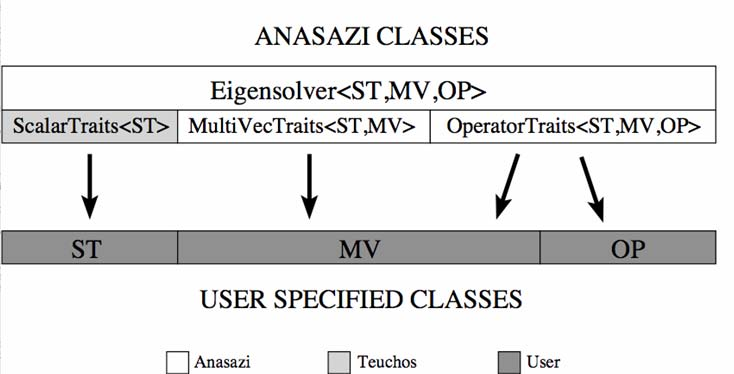
\includegraphics[height=1.5in]{anasazi_linalg_template}
\end{center}
\caption{An eigensolver templated on scalar (ST), multivector (MV), and
operator (OP) type.}
\end{figure}

Another aspect of software reuse that templating alleviates is through the separation of the
eigensolver algorithm from the linear algebra data structures.  This separation, as shown in
Figure \ref{fig:latemplate}, allows a user of the Anasazi framework to leverage an existing 
linear algebra software investment.  All that is required is the template instantiation of the trait
classes, \aspace{MultiVecTraits} and \aspace{OperatorTraits}, for the user-defined multvector 
and operator, respectively.  The \aspace{ScalarTraits} class and respective template 
instantiations for different scalar types are provided by the Trilinos Teuchos package 
\cite{Trilinos:Teuchos}. Another user-friendly aspect of employing templates and traits mechanisms
is that the Anasazi eigensolver, eigenproblem, and eigensolution are all defined by the 
specified scalar, multivector, and operator type at compile time.  This approach, as opposed to
using abstract interfaces and dynamic polymorphism, avoids any dynamic casting of the multivectors 
and operators in the user's interaction with the Anasazi framework.

%eigenvalue algorithm from the linear algebra data structures. The operator type templating
%is analogous to the reverse communication interface used by ARPACK for providing
%matrix-vector products.

%Because the underlying data types are unknown to the Anasazi
%developer, algorithms are developed abstractly. Access to the
%functionality of the underlying objects is provided via the classes
%\aspace{MultiVecTraits} and \aspace{OperatorTraits}. These classes
%implement the traits mechanism~\cite{myer:95} and specify the
%operations that the multivector and operator classes must support in
%order to be used within Anasazi. This mechanism hides the low-level
%details of the underlying data structures.  As a result, a single
%eigensolver implementation in Anasazi can be exploited on a number of
%diverse computing platforms: serial, distributed memory parallel,
%multi-core shared memory parallel, graphics processing units, FPGAs,
%etc.

The \aspace{MultiVecTraits} and \aspace{OperatorTraits} classes specify
the operations that the multivector and operator type must support in order for them to be
used by Anasazi. Through the observations made in Section \ref{sec:algorithm-overview}, 
it is clear that the \aspace{OperatorTraits} class only needs to provide one method,
described in Table \ref{tab:anasazi:opt}, that applies an operator to a multivector.  
This interface defines the only interaction required from an operator, eventhough
the underlying operator may be a matrix, 
spectral transformation, or preconditioner.
\begin{table}[bth]
\begin{center}
  \caption{The method provided by the \aspace{OperatorTraits} interface.}
\label{tab:anasazi:opt}
\begin{tabular}{| p{4cm} | p{8cm} |}
\hline
%%
\multicolumn{2}{|c|}{\textbf{OperatorTraits$<$ST,MV,OP$>$}} \\\hline
\emph{Method name} & \emph{Description} \\\hline
{\tt Apply(A,X,Y)} & Applies the operator $A$ to the multivector $X$, placing the
result in the multivector $Y$. \\
\hline
%%
\end{tabular}
\end{center}
\end{table}

The methods defined by the \aspace{MultiVecTraits} class, listed in
Table~\ref{tab:anasazi:mvt}, are the creational and arithmetic methods necessitated
by the observations in Section \ref{sec:algorithm-overview}.
The creational methods generate empty or populated multivectors from a previously
created multivector. The populated multivectors can be 
a deep copy, where the object contains the storage for the multivector entries, or a shallow copy, 
where the object has a view of another multivector's storage.
A shallow copy is useful when only a
subset of the columns of a multivector is required for computation, which is a situation that 
commonly occurs during the generation of a Krylov subspace. All the creational methods return
a reference-counted pointer \cite{Detlefs:1992:GCR,Teuchos-RCP} to the new multivector (\aspace{RCP<MV>}). 

%This concept provides Anasazi access to the performance benefits
%previously available only to C/FORTRAN implementations.

\begin{table}
\begin{center}
  \caption{The methods provided by the \aspace{MultiVecTraits} interface.}
\label{tab:anasazi:mvt}
\begin{tabular}{| p{4cm} | p{8cm} |}
\hline
%%%
%\multicolumn{2}{|c|}{\textbf{OperatorTraits$<$ST,MV,OP$>$}} \\\hline
%\emph{Method name} & \emph{Description} \\\hline
%Apply($A,X,Y$) & Applies the operator $A$ to the multivector $X$, placing the
%result in the multivector $Y$. \\\hline
%\hline
%%%
\multicolumn{2}{|c|}{\textbf{MultiVecTraits$<$ST,MV$>$}} \\\hline
%%%
\emph{Method name} & \emph{Description} \\\hline
{\tt Clone(X,numvecs)}           & Creates a new multivector from $X$ with
$numvecs$ vectors.  \\

{\tt CloneCopy(X,index)} & Creates a new multivector with a copy of the contents of
a subset of the multivector $X$ (deep copy). \\

{\tt CloneView(X,index)} & Creates a new multivector that shares the selected
contents of a subset of the multivector $X$ (shallow copy).  \\\hline

{\tt GetVecLength(X)} & Returns the vector length of the multivector $X$.
\\

{\tt GetNumberVecs(X)}& Returns the number of vectors in the multivector $X$.
\\\hline

{\tt MvTimesMatAddMv(alpha,X}, & Applies a dense matrix $D$ to multivector $X$ and \\ 
{\tt \ \ \ \ \ \ \ \ \ \ \ \ \ \ \ \ M,beta,Y)} & accumulates the result into multivector $Y$:\\ & $Y \leftarrow \alpha X D + \beta Y$.  \\

{\tt MvAddMv(alpha,X,beta,Y)}  & Performs multivector AXPBY: $Y \leftarrow \alpha X + \beta Y$.
\\

{\tt MvTransMv(alpha,X,Y,D)} & Computes the dense matrix $D \leftarrow \alpha X^H Y$.
\\

{\tt MvDot(X,Y,d)} & Computes the corresponding dot products:
$d[i] \leftarrow X[i]^H Y[i]$.  \\

{\tt MvScale(X,d)}    & Scales the i-th column of a multivector $X$ by $d[i]$. \\

{\tt MvNorm(X,d)}     & Computes the 2-norm of each vector of
$X$: $d[i] \leftarrow \|X[i]\|_2$  \\\hline

{\tt SetBlock(X,Y,index)} & Copies the vectors in $X$ to a subset of vectors in
$Y$. \\

{\tt MvInit(X,alpha)} & Replaces each entry in the multivector $X$ with a scalar $\alpha$.  \\

{\tt MvRandom(X)} & Replaces the entries in the multivector $X$ by random
scalars. \\

\hline
\end{tabular}
\end{center}
\end{table}



The arithmetic methods defined by the \aspace{MultiVecTraits} are essential to the computations
required by the Rayleigh-Ritz method and the general eigen-iteration.  The 
\aspace{MvTimesMatAddMv} and \aspace{MvAddMv} methods are necessary for updating the approximate 
eigenpairs 
in Step~4 of the Algorithm \ref{algo:obliqueRR}
or Step~2 of Algorithm \ref{algo:eigen-iter}.
The \aspace{MvDot} and \aspace{MvTransMv} methods are required by the orthogonalization procedures
utilized in Steps~1 and 3 of the eigen-iteration.  The \aspace{MvScale} and \aspace{MvNorm}
methods are necessary, at the very least, for the computation of approximate eigenpairs and for  
some termination criteria (Step~4) of the eigen-iteration. 
Deflation and locking in Step~3 of the eigen-iteration necessitates the \aspace{SetBlock} method.
Initialization of the bases for the eigen-iteration requires
methods such as \aspace{MvRandom} and \aspace{MvInit}.
The ability to perform error checking and debugging in Anasazi is supported by methods that give 
dimensional attributes (\aspace{GetVecLength}, \aspace{GetNumberVecs}) and allow the users to print
out a multivector (\aspace{MvPrint}). 

Specialization of the \aspace{MultiVecTraits} and \aspace{OperatorTraits} classes on
given template arguments is compulsory for their usage in the eigensolver framework.
However, Anasazi provides the following specializations of these trait classes:
\begin{itemize}
  \item \aspace{Epetra\_MultiVector} and \aspace{Epetra\_Operator} (with scalar type
    \aspace{double}) allow Anasazi to be used with the Epetra~\cite{Trilinos:Epetra} linear
    algebra library provided with Trilinos. This gives Anasazi the ability to interact with 
    Trilinos packages that support the Epetra\_Operator interface, like Amesos, AztecOO, Belos, 
    Ifpack, ML, and NOX/LOCA. 
  \item \aspace{Thyra::MultiVectorBase<ST>} and
    \aspace{Thyra::LinearOpBase<ST>} (with arbitrary scalar type
    \aspace{ST}) allow Anasazi to be used with any classes that implement the abstract interfaces
    provided by the Thyra~\cite{Trilinos:Thyra} package of Trilinos.
%  \item \aspace{MultiVec<ST>} and \aspace{Operator<ST>} (with
%    arbitrary scalar type \aspace{ST}) allow Anasazi to be used with any classes that implement
%    the Anasazi abstract base classes \aspace{MultiVec} and \aspace{Operator}.
\end{itemize}
For scalar, multivector and operator types not covered by the provided specializations,
alternative specializations of \aspace{MultiVecTraits} and \aspace{OperatorTraits}
must be created. One benefit of the traits mechanism is that it does
not require that the data types are C++ classes.  Furthermore, it
does not require modification to existing data types, it only serves as a translator between
the data type's native functionality and Anasazi's required functionality. 


\subsection{The Anasazi Eigensolver Framework}
%%%%%%%%%%%%%%%%%%%%%%%%%%%%%%%%%%%%%%%%%%%%%%%%%%%%%%
\label{subsec:anasazi:solver_framework}

In this section we will discuss how to implement an eigensolver
in Anasazi's framework.  We will demonstrate Anasazi is 
a framework of algorithmic components, where decoupled operations 
simplify component verification, encourage code reuse, and maximize flexibility
in implementation. This modularized approach requires a \emph{solver manager} that
combines a strategy with these algorithmic components to define an eigensolver.
The high-level class collaboration graph for Anasazi's \aspace{SolverManager} class in 
Figure \ref{fig:solverColl} lists all the algorithmic components offered by the Anasazi
framework for implementing an eigensolver.

\begin{figure}[htb]
\label{fig:solverColl}
\begin{center}
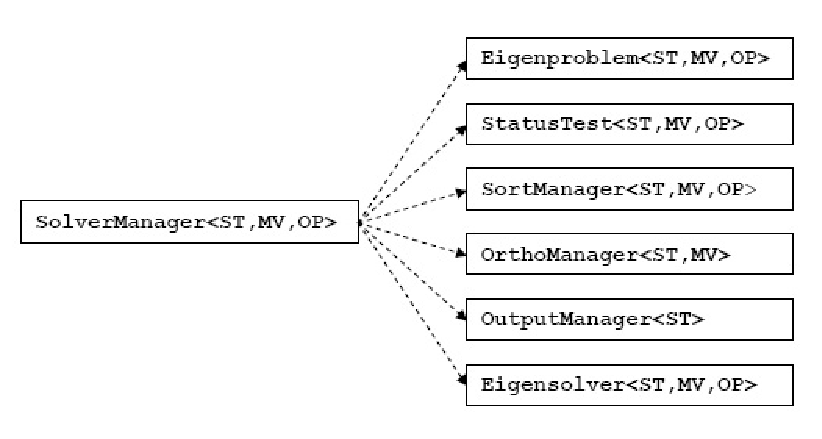
\includegraphics[height=2in]{anasazi_slvr_collaborations.pdf}
\end{center}
\caption{Anasazi::SolverManager class collaboration graph.}
\end{figure}

The first component that is essential to the \aspace{SolverManager} is the 
\aspace{Eigenproblem} class.  \aspace {Eigenproblem} is an abstract class that is a container for 
the components and solution of an eigenvalue problem. By requiring eigenproblems to derive from
\aspace{Eigenproblem}, Anasazi defines a minimum interface that can be expected of all
eigenvalue problems by the classes that will work with these problems. The methods provided
by this interface, shown in Table \ref{tab:anasazi:eigenproblem}, are generic enough to define
an eigenproblem that is standard or generalized, Hermitian or non-Hermitian.  Furthermore, this
interface allows the definition of a preconditioner, for 
preconditioned eigensolvers, as well as the definition of a spectral transformation,
for Arnoldi-based eigensolvers. 
\begin{table}[htb]
\begin{center}
  \caption{A list of methods provided by any derived \aspace{Eigenproblem}.} 
\label{tab:anasazi:eigenproblem}
\begin{tabular}{| p{2cm}  p{2cm} | p{6cm} |}
\hline
\multicolumn{3}{|c|}{\textbf{Eigenproblem$<$ST,MV,OP$>$}} \\\hline
\multicolumn{2}{|c|}{\emph{Method name}} & \emph{Description} \\
\hline
{\tt setOperator()}&{\tt getOperator()}    & Access the operator for which eigenvalues will be computed. \\
{\tt setA()}&{\tt getA()}                  & Access the operator A of the eigenvalue problem $Ax=\lambda Mx$ . \\
{\tt setM()}&{\tt getM()}                  & Access the operator M of the eigenvalue problem $Ax=\lambda Mx$ . \\
{\tt setPrec()}&{\tt getPrec()}            & Access the preconditioner for this eigenvalue problem $Ax=\lambda Mx$ . \\
{\tt setInitVec()}&{\tt getInitVec()}      & Access the initial guess. \\
{\tt setAuxVecs()}&{\tt getAuxVecs()}      & Access the auxiliary vectors. \\
{\tt setNEV()}&{\tt getNEV()}              & Access the number of eigenvalues (NEV) that are requested.  \\
{\tt setHermitian()}&{\tt isHermitian()}   & Access the symmetry of the eigenproblem. \\
{\tt setProblem()}&{\tt isProblemSet()}    & Access whether the eigenproblem is fully defined.  \\
{\tt setSolution()}&{\tt getSolution()}    & Access the solution to the eigenproblem. \\
\hline
\end{tabular}
\end{center}
\end{table}

From a user's perspective, the most important part of the interface may be the methods 
for storing and retrieving the results of the eigenvalue computation:
\begin{verbatim}
const Eigensolution & Eigenproblem::getSolution();
void Eigenproblem::setSolution(const Eigensolution & sol);
\end{verbatim}
The \aspace{Eigensolution} class was developed in order to
facilitate setting and retrieving the solution data from an eigenproblem.  
Furthermore, the \aspace{Eigensolution} class was designed for storing
solution data from both Hermitian and non-Hermitian eigenproblems. 
This structure contains the following information:
\begin{itemize}
  \item \verb!RCP< MV > Evecs! \\
   The computed eigenvectors.
 \item \verb!RCP< MV > Espace! \\
   An orthonormal basis for the computed eigenspace.
 \item \verb!std::vector< Value< ST > > Evals! \\
   The computed eigenvalue approximations.
 \item \verb!std::vector< int > index! \\
   An index scheme enabling compressed storage of eigenvectors for non-Hermitian problems.
 \item \verb!int numVecs! \\
   The number of computed eigenpair approximations.
\end{itemize}
The \aspace{Eigensolution::index} vector has \aspace{numVecs} integer entries that take 
one of three values: $\{0, +1, -1\}$. These values allow the eigenvectors to be retrieved as follows:
\begin{itemize}
  \item \aspace{index[i]== 0}: the $i$-th eigenvector is stored uncompressed in column $i$ of
    \verb!Evecs!.
  \item \aspace{index[i]==+1}: the $i$-th eigenvector is stored compressed, with the real
    component in column $i$ of \verb!Evecs! and the \emph{positive} complex component
    stored in column $i+1$ of \verb!Evecs!
  \item \aspace{index[i]==-1}: the $i$-th eigenvector is stored compressed, with the real
    component in column $i-1$ of \verb!Evecs! and the \emph{negative} complex component
    stored in column $i$ of \verb!Evecs!
\end{itemize}
This storage scheme is only required for non-symmetric problems over the real field and enables
Anasazi to use \aspace{numVecs} vectors to store \aspace{numVecs} eigenvectors, even when
complex conjugate pairs are present.  All other eigenproblems will return an index vector 
composed entirely of zeroes. 
%For the real
%non-symmetric case, the $+1$ index will always immediately precede
%the corresponding $-1$ index.

The \aspace{Value} structure is a simple container, templated on scalar type, that
has two members: the real and imaginary part of an eigenvalue.  The real and imaginary
parts are stored as the magnitude type of the scalar type.  The \aspace{Value} structure
along with the \verb!index! vector enable the \aspace{Eigensolution} structure to 
store the solutions from either real or complex, Hermitian or non-Hermitian eigenvalue
problems. Implementations of the \aspace{SolverManager} class are expected to place the 
results of their computation in the \aspace{Eigenproblem} class using an \aspace{Eigensolution}. 

The second component that is essential to a \aspace{SolverManager} is the \aspace{Eigensolver}
class. The \aspace{Eigensolver} abstract base class defines the basic interface that must be met
by any eigen-iteration class in Anasazi. This class defines two types of methods: status methods and
solver-specific methods. A list of these methods is given in Table~\ref{tab:anasazi:itermethods}.
\begin{table}[htp]
\begin{center}
\caption{A list of methods provided by any derived \aspace{Eigensolver}.} 
\label{tab:anasazi:itermethods}
\begin{tabular}{| p{3cm} | p{6cm} |}
\hline
\multicolumn{2}{|c|}{\textbf{Eigensolver$<$ST,MV,OP$>$}} \\\hline
\multicolumn{2}{|c|}{\emph{Status Methods}} \\
\hline
\emph{Method name} & \emph{Description} \\
\hline
{\tt getNumIters()}       & current number of iterations. \\
{\tt getRitzValues()}     & most recent Ritz values. \\
{\tt getRitzVectors()}    & most recent Ritz vectors. \\
{\tt getRitzIndex()}      & Ritz index needed for indexing compressed Ritz vectors. \\
{\tt getResNorms()}       & residual norms, with respect to the \aspace{OrthoManager}. \\
{\tt getRes2Norms()}      & residual Euclidean norms. \\
{\tt getRitzRes2Norms()}  & Ritz residual  Euclidean norms. \\
{\tt getCurSubspaceDim()} & current subspace dimension. \\
{\tt getMaxSubspaceDim()} & maximum subspace dimension. \\
{\tt getBlockSize()}      & block size. \\
\hline
\multicolumn{2}{|c|}{\emph{Solver-specific Methods}} \\
\hline
\emph{Method name} & \emph{Description} \\
\hline
{\tt getState()}       & returns a specific structure with read-only pointers to
                       the current state of the solver. \\
{\tt initialize()}     & accepts a solver-specific structure enabling the user to initialize
                       the solver with a particular state.\\
{\tt iterate()}        & performs eigen-iteration until the status test indicates the need
                       to stop or an error occurs.\\
\hline
\end{tabular}
\end{center}
\end{table}
The status methods are defined by the \aspace{Eigensolver}
abstract base class and represent the information about the iteration status that can 
be requested from any eigensolver.  Each eigensolver iteration also provides low-level, 
solver-specific methods for accessing and setting the state of the solver.  
An eigensolver's state is stored in a solver-specific structure and is expected to fully describe 
the current state of the solver or the state the solver needs to be initialized to.  
A simple example of a state structure can be seen in Figure \ref{fig:state}.
\begin{figure}[htb]
\begin{center}
\begin{boxedverbatim}
  template <class ST, class MV>
  struct SomeEigensolverState {
    /* The current dimension of the subspace.
     * NOTE: This should always be equal to SomeEigensolver::getCurSubspaceDim()
    int curDim;
    /* The current subspace. */
    RCP<const MV> V;
    /* The current Rayleigh-Ritz projection */
    RCP<const Teuchos::SerialDenseMatrix<int,ST> > H;
    SomeEigensolverState() : curDim(0), V(Teuchos::null),
                             H(Teuchos::null) {}	
  };
\end{boxedverbatim}
\end{center}
\caption{Example of an \aspace{Eigensolver} state structure.}
\label{fig:state}
\end{figure}

The eigensolver iterations implemented using the \aspace{Eigensolver} class
are generic iteration kernels that do not have the intelligence to determine when
to stop the iteration, what the eigenvalues of interest are, where to send output,
or how to orthogonalize the basis for a subspace.  The intelligence to perform these four
tasks is, instead, provided by the \aspace{StatusTest}, \aspace{SortManager},
\aspace{OutputManager}, and \aspace{OrthoManager} objects, which are passed into the
constructor of an \aspace{Eigensolver} (Figure \ref{fig:constructor}).  This allows 
each of these four tasks to be modified without affecting the basic eigensolver 
iteration. When combined with the status and state-specific \aspace{Eigensolver} 
methods, this provides the user with a large degree of control over eigensolver iterations.
\begin{figure}[htb]
\begin{center}
\begin{boxedverbatim}
Eigensolver(
   const RCP< Eigenproblem<ST,MV,OP> > &problem,
   const RCP< SortManager<ST,MV,OP>  > &sorter,
   const RCP< OutputManager<ST>      > &printer,
   const RCP< StatusTest<ST,MV,OP>   > &tester,
   const RCP< OrthoManager<ST,OP>    > &ortho,
   ParameterList                       &params
 );
\end{boxedverbatim}
\end{center}
\caption{Basic constructor for an \aspace{Eigensolver}}
\label{fig:constructor}
\end{figure}

The abstract \aspace{StatusTest} class is used to provide the interface for stopping 
conditions for an eigen-iteration. There are numerous conditions under which an eigen-iteration 
should be stopped, the most common are the number of iterations, convergence, and deflation.
Often the decision to stop an eigensolver iteration is based on a hierarchy 
of problem-dependent, logically connected stopping conditions.
This, possibly complex, reasoning does not have to be known by the \aspace{Eigensolver} class,
which queries the \aspace{StatusTest} during its class method \aspace{iterate()} to determine 
whether or not to continue iterating (Figure~\ref{fig:comm}).
\begin{figure}[htb]
\begin{center}
\begin{boxedverbatim}
SomeEigensolver::iterate() {
  while ( somestatustest.checkStatus(this) != Passed ) {
    //
    // perform eigensolver iterations
    //
  }
  return;  // return back to caller
}
\end{boxedverbatim}
\end{center}
\caption{Example of communication between status test and eigensolver}
\label{fig:comm}
\end{figure}
The \aspace{StatusTest} class provides a method, \verb!checkStatus()!, which queries the methods provided by
\aspace{Eigensolver} and determines whether the solver meets the criteria defined by a particular 
status test. After a solver returns from \verb!iterate()!, the caller has the ability to access the
solver's state and the option to re-initialize the solver with a new state and continue iterating.

A \aspace{StatusTest} is a desirable feature in the Anasazi software framework because it
provides the eigensolver user and developer with a flexible interface for interrogating the eigen-iteration.
Besides the basic usage, this interface makes it possible to select stopping conditions at runtime 
and it also makes it possible to put hooks in the eigensolver for debugging and checkpointing.
This flexible approach to selecting and developing stopping criteria for an eigensolver is not
available in PRIMME or SLEPc.  Since the user provides the memory for computations, ARPACK can give the
user the power to determine if an iteration should terminate.  However, this is not a clean, direct 
approach because the user must know the data layout to determine where the information is for making
this decision.

The purpose of the \aspace{SortManager} class is to separate the \aspace{Eigensolver} from the sorting
functionality, giving users the opportunity to choose the eigenvalues of interest in whatever manner is
deemed to be most appropriate. Anasazi defines an abstract class \aspace{SortManager} with
two methods, one for sorting real values and one for sorting complex values, shown in Figure \ref{fig:sort}
The \aspace{SortManager} is also expected to provide the permutation vector if the 
\aspace{Eigensolver} passes a non-null pointer for \verb!perm! to the \aspace{sort} method.  This is 
necessary, because many eigen-iterations must sort their approximate eigenvectors, as well as their 
eigenvalues.
\begin{figure}[htb]
\begin{center}
\begin{boxedverbatim}
// Sort n real values stored in evals and return permutation, if required, in perm.
void sort(Eigensolver<ST,MV,OP>* solver, 
          const int n, 
          std::vector<typename Teuchos::ScalarTraits<ST>::magnitudeType> &evals,
          std::vector<int> *perm) 
// Sort n complex values, whose real and imaginary part are stored in r_evals 
//   and i_evals, respectively. Return permutation, if required, in perm.
void sort(Eigensolver<ST,MV,OP>* solver, 
          const int n, 
          std::vector<typename Teuchos::ScalarTraits<ST>::magnitudeType> &r_evals, 
          std::vector<typename Teuchos::ScalarTraits<ST>::magnitudeType> &i_evals, 
          std::vector<int> *perm)
\end{boxedverbatim}
\end{center}
\caption{Example of communication between status test and eigensolver}
\label{fig:sort}
\end{figure}



\begin{table}[htp]
\begin{center}
\caption{A list of methods provided by any derived \aspace{OrthoManager}.} 
\label{tab:anasazi:orthomanager}
\begin{tabular}{| p{4cm} | p{6cm} |}
\hline
\multicolumn{2}{|c|}{\textbf{OrthoManager$<$ST,MV$>$}} \\\hline
\emph{Method name} & \emph{Description} \\
\hline
{\tt innerProd(X,Y,Z)} &
Provides the inner product defining the concepts of orthogonality: $Z = \langle X, Y \rangle$ \\
{\tt norm(X,normvec)} &
Provides the norm norm induced by the inner product: $normvec[i] = \sqrt{\langle X[i], Y[i] \rangle}$\\
{\tt project(X,Q,C) } &
Projects the multivector X onto the subspace orthogonal to the multivectors Q, optionally returning the coefficients of 
X with respect to the Q.\\
{\tt normalize(X,B)} &
Computes an orthonormal basis for the multivector X, optionally returning the coefficients
of X with respect to the computed basis.\\
{\tt projectAndNormalize(X,Q,C,B)} &
Projects the multivector X onto the subspace orthogonal to the multivectors Q and computes an orthonormal basis (orthogonal to the Q) 
for the resultant, optionally returning the coefficients of X with respect to the Q and the computed basis.\\
\hline
\end{tabular}
\end{center}
\end{table}



Since orthogonalization and orthonormalization are commonly performed
computations in iterative eigensolvers and can be implemented in a variety of ways, 
the \aspace{OrthoManager} class separates the \aspace{Eigensolver}
from this functionality. The \aspace{OrthoManager} defines a small number of
orthogonalization-related operations, including choice of an inner
product.

// START HERE!!!
As explained in Section
\ref{sec:algorithm-overview}, all our current implementations are
orthogonal Rayleigh-Ritz methods where an orthonormal basis
representation is computed. 
Combined with the plethora of available methods for
performing these computations, Anasazi has left as much leeway to
the users as possible. To this end, Anasazi provides two concrete
orthogonalization managers:
\begin{itemize}
\item
  \aspace{BasicOrthoManager} - performs orthogonalization using
  multiple steps of classical Gram-Schmidt \cite{dgks:76}.
\item
  \aspace{SVQBOrthoManager} - performs orthogonalization using the
  SVQB orthogonalization technique described by Stathapoulos and
  Wu~\cite{Stathopoulos:2002:BOP}.
\end{itemize}

\cbcomm{emphasize: solver managers driven by parameter lists.}

While this approach to interfacing with the solver is powerful, it can be overwhelming. It
requires the user to construct a number of support classes and to manage calls to
\verb!Eigensolver::iterate()!. The \aspace{SolverManager} class was developed to
encapsulate an instantiation of \aspace{Eigensolver}, providing additional functionality
and handling low-level interaction with the eigensolver that a user may not want to
specify. Solver managers are intended to be easy to use, while still providing the
features and flexibility needed to solve large-scale eigenvalue problems.

For example, the constructor of \aspace{BlockDavidsonSolMgr} accepts only two arguments:
an \aspace{Eigenproblem} specifying the eigenvalue problem to be solved and a
\texttt{ParameterList} of options specific to this solver manager. This solver manager
instantiates a \aspace{BlockDavidson} subclass of \aspace{Eigensolver}, along with the
status tests and other support classes needed by the eigensolver, as
specified by the parameter list. To solve the eigenvalue
problem, the user simply calls the \verb!solve()! method of \aspace{BlockDavidsonSolMgr}.
The solver manager calls \verb!iterate()!, performs restarts and locking, and places the
final solution into the \aspace{Eigenproblem}.

Under this framework, users have a number of options for performing eigenvalue
computations with Anasazi:
\begin{itemize}
\item
Use an existing solver manager. In this case, the user is limited to
the functionality provided by the existing solver managers.
\item
Develop a new solver manager for an existing eigensolver.
The user can extend the functionality provided by the eigensolver,
specifying custom configurations for status tests,
orthogonalization, restarting, locking,  etc.
\item
Implement a new eigensolver (and so extend Anasazi). The user can
write an eigensolver for an iteration that is not represented in
Anasazi. The user still has the benefit of the support classes
provided by Anasazi, and the knowledge that this effort can be
easily employed by anyone already familiar with Anasazi.
\end{itemize}


\subsection{Anasazi Classes}
%%%%%%%%%%%%%%%%%%%%%%%%%%%%%%%%%%%%%%%%%%%%%%%%%%%%%%
\label{subsec:anasazi:classes}

Anasazi is designed with extensibility in mind, so that users can
augment the package with any special functionality that may be
needed. However, the released version of Anasazi provides all
functionality necessary for solving a wide variety of problems. This
section lists and briefly describes the classes used in Anasazi.

Anasazi provides users with a concrete implementation of
\aspace{Eigenproblem}, called \aspace{BasicEigenproblem}. This basic implementation
provides all the functionality necessary to describe both generalized and standard,
Hermitian and non-Hermitian linear eigenvalue problems.

However, a user working
directly with an eigensolver (i.e., not with a solver manager) will need to recover the
solution directly from the eigensolver state.

%The eigenvalues are always stored as two real values, even
%when templated on a complex data type or when the eigenvalues are
%real. Similarly, a basis for the eigenspace can always be represented
%by a multivector of width \verb!numVecs!, even for non-symmetric
%eigenproblems over the real field. However, the storage scheme for
%eigenvectors requires more finesse.

%When solving real symmetric eigenproblems, the eigenvectors can always
%be chosen to be real, and therefore can be stored in a single column
%of a real multivector. When solving eigenproblems over a complex
%field, whether Hermitian or non-Hermitian, the eigenvectors may be
%complex, but the multivector is defined over the complex field, so
%that this poses no problem. However, real non-symmetric problems can
%have complex eigenvectors, which prohibits a one-for-one storage
%scheme using a real multivector.  Fortunately, the eigenvectors in
%this scenario occur as complex conjugate pairs, so the pair can be
%stored in two real vectors. This permits a compressed storage scheme,
%which uses an index vector stored in the \aspace{Eigensolution},
%allowing conjugate pair eigenvectors to be easily retrieved from
%\verb!Evecs!.

%\begin{remark}
%  Solver managers all put the computed eigensolution into the eigenproblem class before
%  returning from \verb!solve()!. Eigensolvers do not; a user working directly with an
%  eigensolver will need to recover the solution directly from the eigensolver state.
%\end{remark}


% powerful, but can be tedious. Solver managers provide a way for users
% to encapsulate specific solving strategies inside of an easy-to-use
% class. Novice users may prefer to use existing solver managers, while
% advanced user may prefer to write custom solver managers.

\aspace{SolverManager} defines only two methods: a constructor
accepting an \aspace{Eigenproblem} and a parameter list of
options specific to the solver manager; and a \verb!solve()! method, taking no
arguments and returning either \aspace{Converged} or
\aspace{Unconverged} (Figure~\ref{fig:examplesolve}).

\begin{figure}[htb]
\begin{center}
\begin{boxedverbatim}
// create an eigenproblem
RCP< Anasazi::Eigenproblem<ST,MV,OP> > problem = ...;
// create a parameter list
ParameterList params;
params.set(...);
// create a solver manager
Anasazi::BlockDavidsonSolMgr<ST,MV,OP> solman(problem,params);
// solve the eigenvalue problem
Anasazi::ReturnType ret = solman.solve();
// get the solution from the problem
Anasazi::Eigensolution<ST,MV> sol = problem->getSolution();
\end{boxedverbatim}
\end{center}
\caption{Sample code for solving an eigenvalue problem using a \aspace{SolverManager}}
\label{fig:examplesolve}
\end{figure}

The goal of the solver manager is to instantiate a subclass of \aspace{Eigensolver}, along
with the necessary support objects. Another purpose of many solver managers is to manage
and initiate the repeated calls to the underlying solver's \verb!iterate()! method. For
solvers that increase the dimension of trial and test subspaces (e.g., Davidson and Krylov
subspace methods), the solver manager may also assume the task of restarting (so that
storage costs may be fixed). This decoupling of restarting from the eigensolver is
beneficial due to the numerous restarting techniques in use.

% These examples are meant to illustrate the flexibility that specific
% solver managers may have in implementing the \verb!solve()! routine.
% Some of these options might best be incorporated into a single
% solver manager, which takes orders from the user via the parameter
% list given in the constructor. Some of these options may better be
% contained in multiple solver managers, for the sake of code
% simplicity. It is even possible to write solver managers that
% contain other solvers managers; motivation for something like this
% would be to select the optimal solver manager at runtime based on
% some expert knowledge, or to create a hybrid method which uses the
% output from one solver manager to initialize another one.

Performing an eigen-iteration requires a number of support classes.  These are passed
through the objects constructor, defined by \aspace{Eigensolver} to take the form listed
in Figure~\ref{fig:constructor}.

These support classes are employed for the following purposes:
\begin{itemize}
  \item \verb!problem! - the eigenproblem to be solved; problem operators are
  defined.
  \item \verb!sorter! - the sort manager selects the
  eigenvalues of interest.
  \item \verb!printer! - the output manager dictates the verbosity level in addition to
    processing output streams.
  \item \verb!tester! - the status tester dictates the termination of the iteration
  \verb!iterate()!.
  \item \verb!ortho! - the orthogonalization manager defines the inner product
   in addition to performing orthogonalization for the solver.
  \item \verb!params! - the parameter list specifies eigensolver-specific
  options.
\end{itemize}

The purpose of the \aspace{StatusTest} is to give the user or solver
manager flexibility in terminating the eigensolver iterations in
order to interact directly with the solver. For instance, typical
reasons for terminating the iteration are:
\begin{itemize}
  \item some convergence criterion has been satisfied;
  \item some portion of the subspace has reached sufficient accuracy to be
  deflated from the iterate or locked;
  \item the solver has performed a sufficient number of iterations.
\end{itemize}
The variation that exists for monitoring these and other conditions requires an abstract mechanism
controlling the iteration.

The following is a list of Anasazi-provided status tests:
\begin{itemize}
  \item \aspace{StatusTestMaxIters} - monitors the number of iterations
    performed by the solver; it can be used to halt the solver at some maximum number of iterations
    or even to require some minimum number of iterations.
  \item \aspace{StatusTestResNorm} - monitors the residual norms of the
    current iterate.
  \item \aspace{StatusTestOrderedResNorm} - monitors the residual
    norms of the current iterate, but only considers the residuals associated with the
    most significant eigenvalues.
  \item \aspace{StatusTestCombo} - a boolean combination of
    other status tests, creating near unlimited potential for complex status tests.
  \item \aspace{StatusTestOutput} - a wrapper around another
    status test, allowing for printing of status information on a call to
    \verb!checkStatus()!.
\end{itemize}

%Anasazi
%provides a concrete implementation called \aspace{BasicSort}.  This class provides basic
%functionality for selecting significant eigenvalues: by largest or smallest real part, by
%largest or smallest imaginary part, or by largest or smallest magnitude.

In order to perform the Rayleigh-Ritz analysis used by the
algorithms illustrating this section, Anasazi utilizes the classes
\aspace{Teuchos::BLAS} and \aspace{Teuchos::LAPACK}. The purpose of
these classes is to provide templated interfaces to the dense linear
algebra routines provided by the BLAS and LAPACK libraries.
Therefore, even such operations as dense matrix-matrix
multiplication are made independent of the scalar field defining the
eigenvalue problem. Users are therefore currently limited to
algorithms provided by LAPACK.

\section{Benchmarking}
%%%%%%%%%%%%%%%%%%%%%%%%%%%%%%%%%%%%%%%%%%%%%%%%%%%%%%
\label{sec:benchmarking}

\begin{table}
\caption{Comparing the overhead of Anasazi with ARPACK; ``---'' denotes a measurement
below the clock resolution.}
\label{table:timings}
\begin{center}
\begin{tabular}{r|ll|ll|}
       \cline{2-5} %\hline
       % after \\: \hline or \cline{col1-col2} \cline{col3-col4} ...
        & \multicolumn{4}{c|}{Computing $50$ Arnoldi vectors} \\ \cline{2-5}
        & \multicolumn{2}{c|}{Matrix-vector time [s]} &
       \multicolumn{2}{c|}{Total runtime [s]}\\ \hline
       Matrix size & ARPACK & Anasazi & ARPACK & Anasazi \\ \hline %\cline{2-5}
       %2500 & 0.010 & 0.018 & 0.47 & 0.54 \\
       10000 & --- & 0.01 & 0.14 & 0.15 \\
       62500 & 0.04 & 0.09 & 1.20 & 1.17 \\
       250000 & 0.15 & 0.32 & 4.98 & 4.79 \\
       1000000 & 0.66 & 1.23 & 19.2 & 18.8 \\
       \hline
        & \multicolumn{4}{c|}{Computing $100$ Arnoldi vectors} \\ \cline{2-5}
        & \multicolumn{2}{c|}{Matrix-vector time [s]} &
       \multicolumn{2}{c|}{Total runtime [s]}\\ \hline
       Matrix size & ARPACK & Anasazi & ARPACK & Anasazi \\ \hline %\cline{2-5}
       %2500 & 0.010 & 0.018 & 0.47 & 0.54 \\
       10000 & 0.03 & 0.02 & 0.53 & 0.55 \\
       62500 & 0.03 & 0.17 & 4.37 & 4.29 \\
       250000 & 0.34 & 0.64 & 17.8 & 17.5 \\
       1000000 & 1.27 & 2.40 & 68.4 & 67.1 \\
       \hline
        & \multicolumn{4}{c|}{Computing $150$ Arnoldi vectors} \\ \cline{2-5}
        & \multicolumn{2}{c|}{Matrix-vector time [s]} &
       \multicolumn{2}{c|}{Total runtime [s]}\\ \hline
       Matrix size & ARPACK & Anasazi & ARPACK & Anasazi \\ \hline %\cline{2-5}
       %2500 & 0.010 & 0.018 & 0.47 & 0.54 \\
       10000 & 0.03 & 0.04 & 1.15 & 1.22 \\
       62500 & 0.14 & 0.26 & 9.53 & 9.39 \\
       250000 & 0.50 & 0.96 & 38.1 & 38.0 \\
       1000000 & 1.97 & 3.56 & 149 & 146 \\
       \hline
     \end{tabular}
\end{center}
\end{table}

The benefits of an object-oriented eigensolver framework such as
Anasazi are manifold: modularization provides improved code reuse,
static polymorphism via templating allows easier code maintenance and
a larger audience, and dynamic polymorphism via inheritance allows
flexible runtime behavior. However, none of these benefits should come
at the expense of code performance. Concern over overhead has long
been an inhibiting factor in the adoption of object-oriented
programming paradigms in scientific computing scenarios. 

We now discuss the important issue of comparing Anasazi and ARPACK
on a model problem. Our interest is in assessing any overhead of
Anasazi and ARPACK, C++ and FORTRAN 77 software.

We benchmarked Anasazi's \aspace{BlockKrylovSchurSolMgr} (with a block size
of one) and ARPACK's \aspace{dnaupd} that compute approximations to the
eigenspace of a non-symmetric matrix. Our goal was to benchmark the
cost of computing $50, 100, 150$ Arnoldi vectors for a finite
difference approximation to a two dimensional convection diffusion
problem. Both codes use the DGKS \cite{dgks:76} method for
maintaining the numerical orthogonality of the Arnoldi basis
vectors.  The Intel 9.1 C++ and FORTRAN compilers were used with
compiler switches ``-O2 -xP'' on an Intel Pentium D, 3GHz, 1MB L2
cache, 2GB main, Linux/FC5 PC.

\cbcomm{rewrite this operator}

The operator application in Anasazi records approximately twice as much time as the ARPACK
implementation. This is because the Anasazi code used an Epetra sparse matrix
representation, while the ARPACK implementation applies the block tridiagonal
matrix via a stencil. Note that the operator application comprised only a small
portion of the clock time in these tests. The performance of the Anasazi library in
computing the Arnoldi vectors is similar to that of ARPACK. Our conclusion is that a
well-designed library in C++ is as efficient as a FORTRAN 77 library.

\section{Conclusion}

\cbcomm{reinforce their clarity}

\cbcomm{issues yet to be handled: anasazi provides only three
eigensolvers, it also provides a framework capable of implementing
multiple eigensolvers. for example, eigen-iterations requiring an
iteration have been implemented using anasazi, such as RTR, TRACEMIN
and Jacobi-Davidson.}

\section{Acknowledgments}
We thank Roscoe Bartlett, Mike Heroux, Roger Pawlowski, Eric Phipps,
and Andy Salinger for many helpful discussions.

\bibliography{anasazi-toms}
\bibliographystyle{acmtrans}


\begin{received}
%????
\end{received}


\end{document}
